\section{Closed-loop Model Checking With Abstraction Tree}
%\subsection{Heart Model Abstraction Tree}
A set of heart models corresponding to different heart conditions are first developed. 
The list can be expanded as new heart conditions are discovered.
Because we start from a set of initial models, and each one may be abstracted using a number of abstraction rules, we have a choice of which rules to apply to which models, and the order in which to apply them.
Depending on which rule is applied when, we end up with different abstract models.
Thus an \emph{abstraction tree} $T_{HM}$ for the heart is created, as shown in \figref{HM_abs}. 
%Note that applying rules in different order results different abstraction tree. 
%The order used to obtain $HM\_tree$ is based on the domain knowledge that certain heart conditions may have similar behaviors and similar inputs to the pacemaker. 
%This systematic grouping maintains the physiological-relevance of the heart model even at higher abstraction levels, and reduce the necessity to resolve ambiguities at lower abstraction levels when model checking certain requirements.
\begin{figure}[!t]
	\centering
	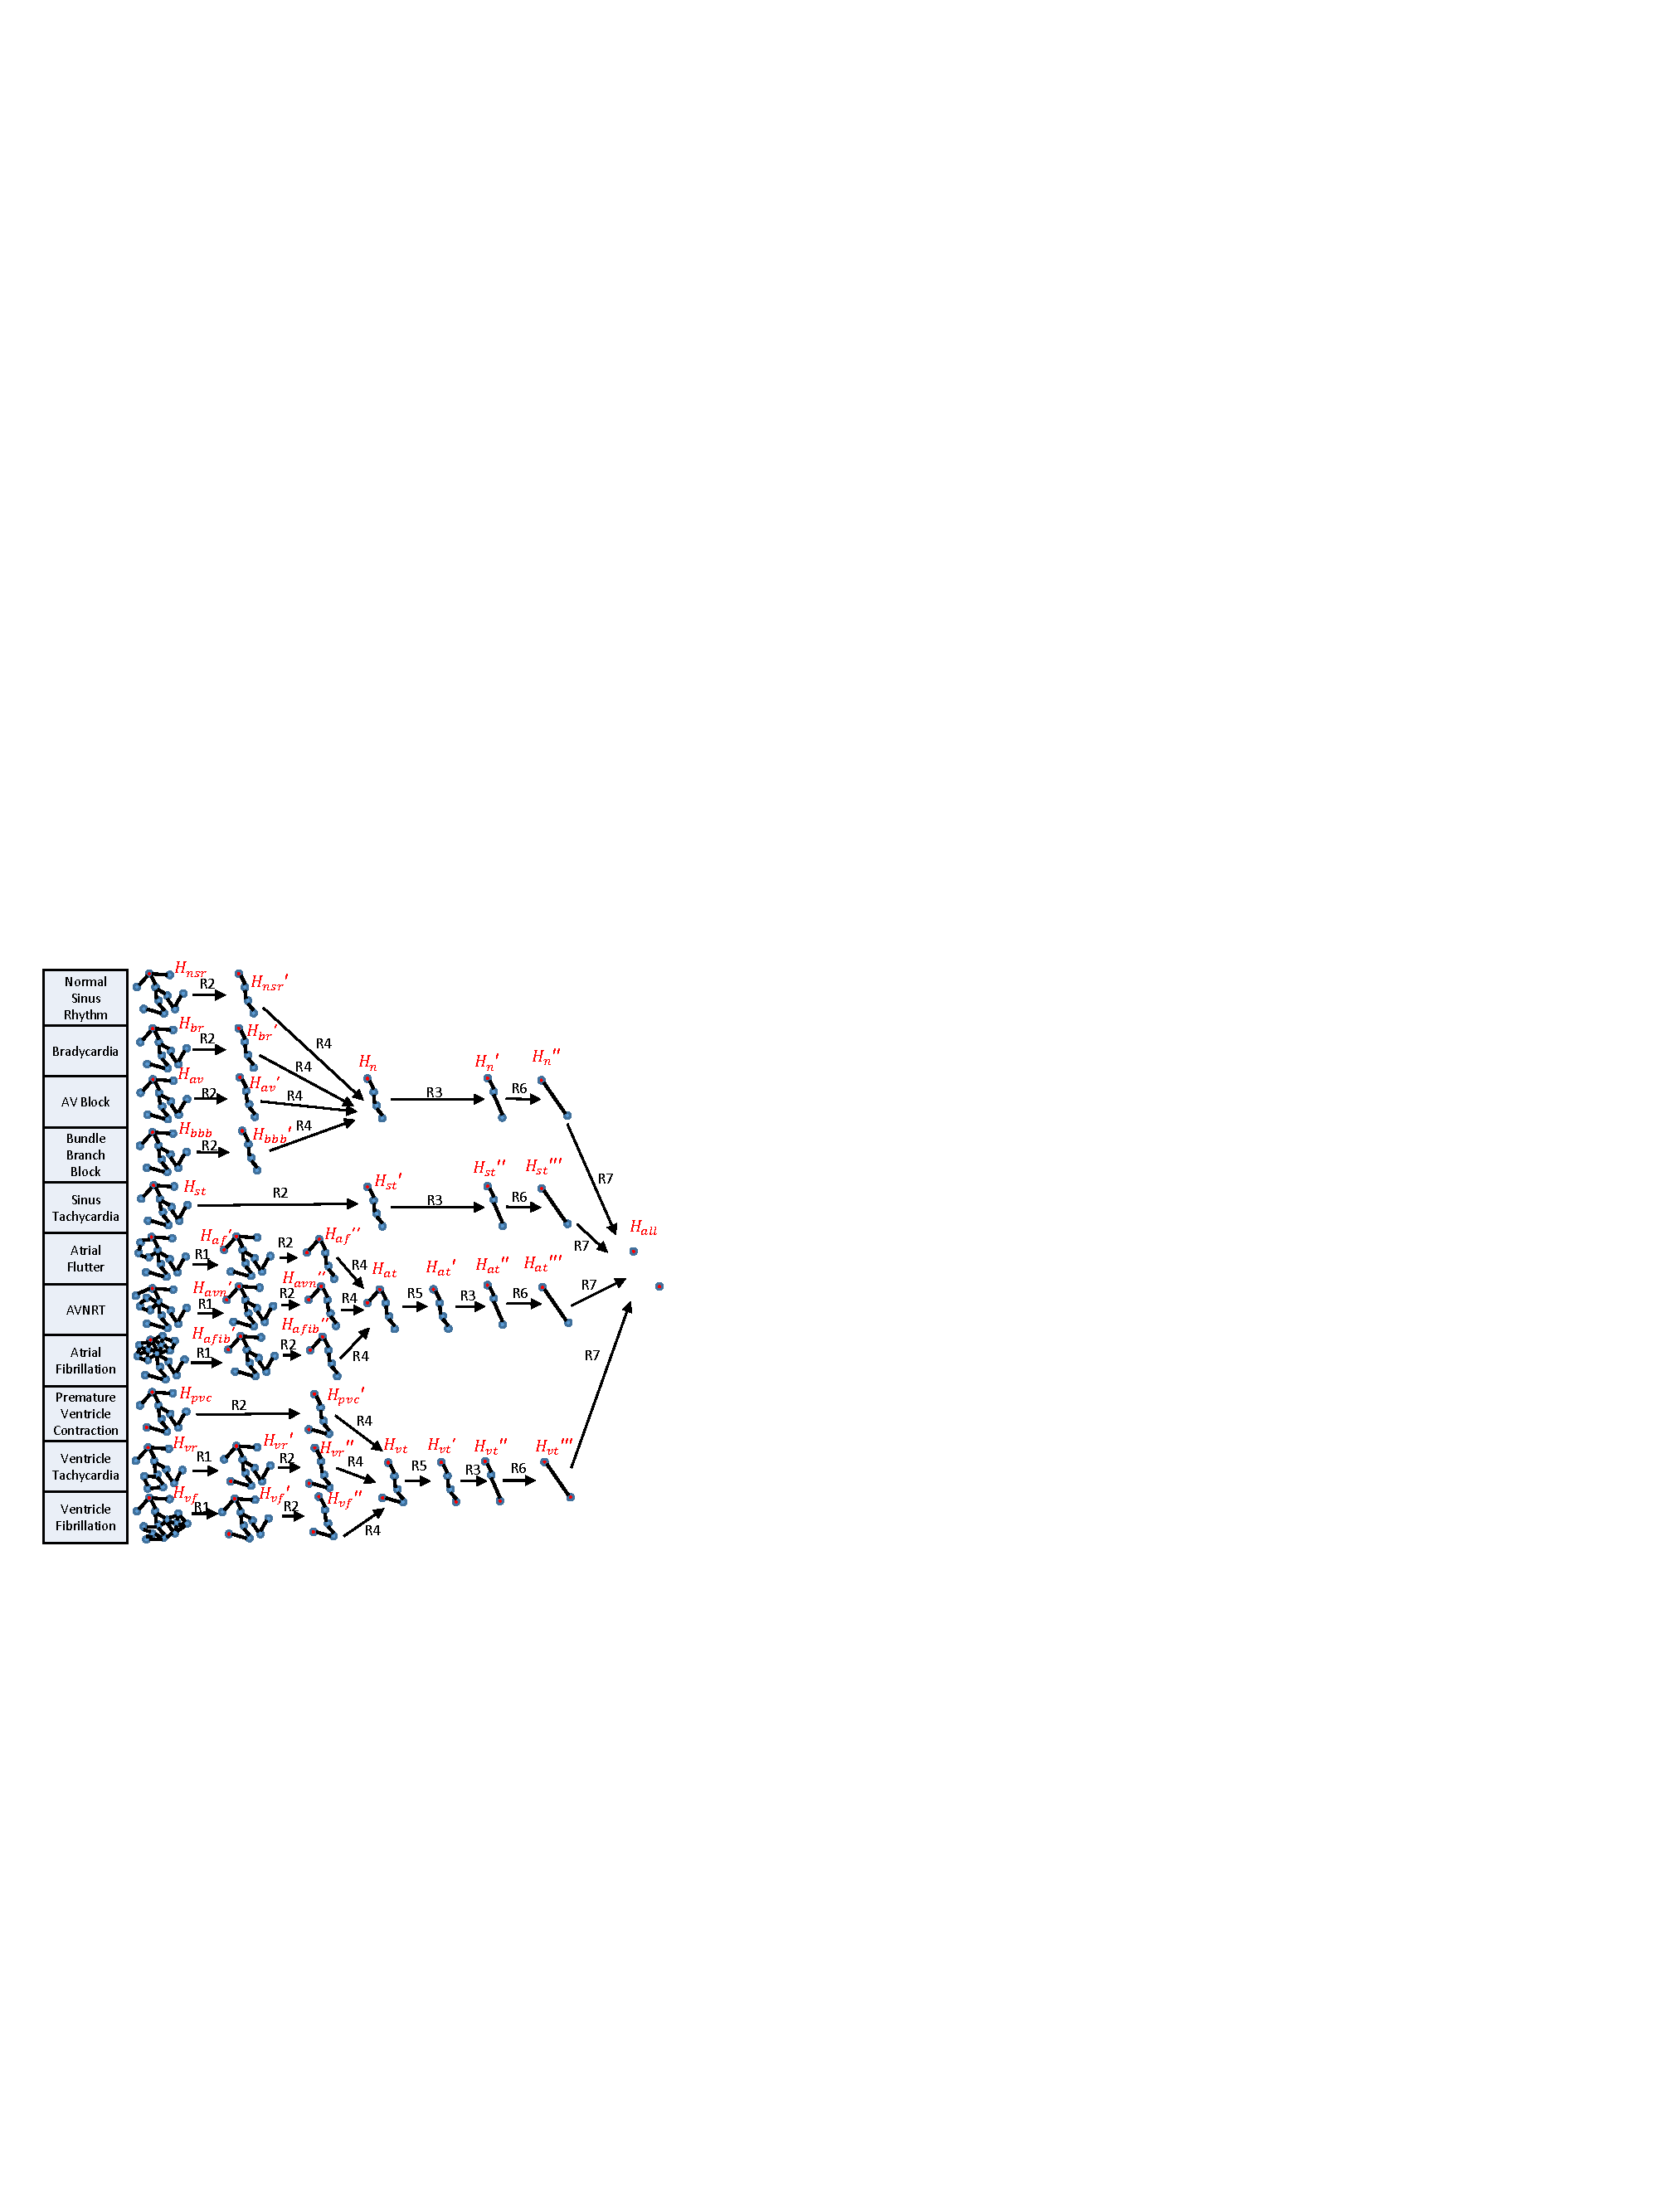
\includegraphics[width=0.85\textwidth]{figs/abs.pdf}
	%\vspace{-5pt}
	\caption{\small Heart Model Abstraction Tree}
	\vspace{-15pt}
	\label{fig:HM_abs}
\end{figure}
%\subsection{Model Checking Procedure}
After the abstraction tree is built, it can be used for closed-loop model checking by non-domain experts. 
The question is which models to select from the abstraction tree to perform model checking, and provide the most concrete counter-examples.
These counter-examples are provided to the physicians, along with the heart models that generated them, to determine their physiological validity.

We now summarize the model checking procedure, and give a detailed example in the next section.
Recall the definition of appropriateness from Section \ref{preliminaries}.
In the technical report \cite{regar_tech}, we show that a sufficient condition for a model $M$ to be appropriate for a requirement $\varphi$ with monitor $Mon$ is
$Var(\varphi) \subset Var(M) \cup Var(Mon)$.
\ifthenelse{\boolean{TECH_REPORT}}{\begin{proof}
	\newcommand{\hs}{\hat{s}}
	To prove that $Var(\varphi) \subset Var(M)$ is a sufficient condition for appropriateness, we introduce some standard terminology.
	For an integer $n \geq 1$, $[n] = \{1,\ldots,n\}$.
	Given a tuple $(a_1,a_2,\ldots,a_n)$ and a subset $H \subset [n]$, the projection function $\proj{}{H}$ retains the components indexed by $H$. E.g., $\proj{(a_1,a_2,a_3)}{1,3} = (a_1,a_3)$.
	
	Let $\Vc = \{V_1,\ldots, V_n\}$ be variables with valuation domains $D_1,\ldots,D_n$, respectively. 
	Let $D = D_1 \times \ldots D_n$ be the state space.
	Let $AP$ be the set of atomic propositions on $\Vc$, i.e. expressions involving the variables in $\Vc$.
	We write $Var(p)$ for the variables that appear in a given proposition $p$, and $Var(\varphi) = \cup_{p \textrm{ in } \varphi} Var(p)$.
	We define the map $\Oc: AP \rightarrow 2^D$ which assigns to each atomic proposition $p$ a subset $\Oc(p)$ of states where the proposition holds.
	Conversely, $\Oc^{-1}(\{s\})$ is the set of atomic propositions that hold for a state $s \in D$.

	Given a proposition $p$, if a variable $v_1$ is not in $Var(p)$, then $\proj{\Oc(p)}{1} = D_1$.
	I.e., $p$ places no constraints on the value of variable $v_1$.
	Given a trace $x = s_0 s_1 s_3 \ldots \in D^\omega$, we define a \emph{run} for $x$ to be the sequence $p_o p_1 p_2 \ldots$ of atomic propositions such that $p_i \in \Oc^{-1}(s_i)$.
	Let $\varphi$ be a formula on $AP$.
	If two traces $x$ and $y$ have the same run and $x \models \varphi$, then $y \models \varphi$.
	
	All our abstraction rules are projections: i.e., associated to each abstraction function $\absfun$ is a set $H \subset [n]$ of indices such that to for every $s = (a_1,a_2,\ldots,a_n) \in D$, $h(s) = \proj{s}{H}$.
	For rule $\absfun_4$, $H = [n]$.
	
	Now let $M$ be a model, 
	$\absfun = \proj{\cdot}{2,\ldots,n}$, and $M' = h(M)$.
	Suppose that $Var(\varphi) \subset Var(M')$.
	Let $x \in \beh(M')$ such that
	\[x = \hs_0 \hs_1 \hs_2 \ldots \models \varphi\] 
	We want to prove that for any $y \in \absfun^{-1}(x)$, $y \models \varphi$.
	First note that $\hs_i \in D_2 \times \ldots \times D_n$.
	Let $p_0 p_1 p_2 \ldots$ be the run corresponding to $x$.
	By definition of run,
	 $\hs_i \in \Oc(p_i) \cap \proj{D}{2,\ldots,n} = \proj{\Oc(p_i)}{2,\ldots,n}$.
	Since $v_1 \notin Var(M')$, then $v_1 \notin Var(p_i)$ for all $p_i$ in $\varphi$.
	Therefore 
	\[\Oc(p_i) = D_1 \times \proj{\Oc(p_i)}{2,\ldots,n}\; \forall i\]
	For any $y \in \absfun^{-1}(x)$, $y = s_0 s_1 s_2 \ldots$ where $s_i = (a_i, \hs_i) \in D$.
	Thus $s_i \in \Oc(p_i)$, which means that $p_0 p_1 \ldots$ is a run of $y$ as well.
	Therefore, $y \models \varphi$.
	
	
	
	
	\end{proof}
	}{}

A search algorithm is developed to select the most abstract models from the abstraction tree $T_{HM}$ that are appropriate for a requirement $Req$. 
The detailed implementation of the algorithm can be found in \cite{regar_tech}.
%\begin{figure}[!t]
		%\centering
		%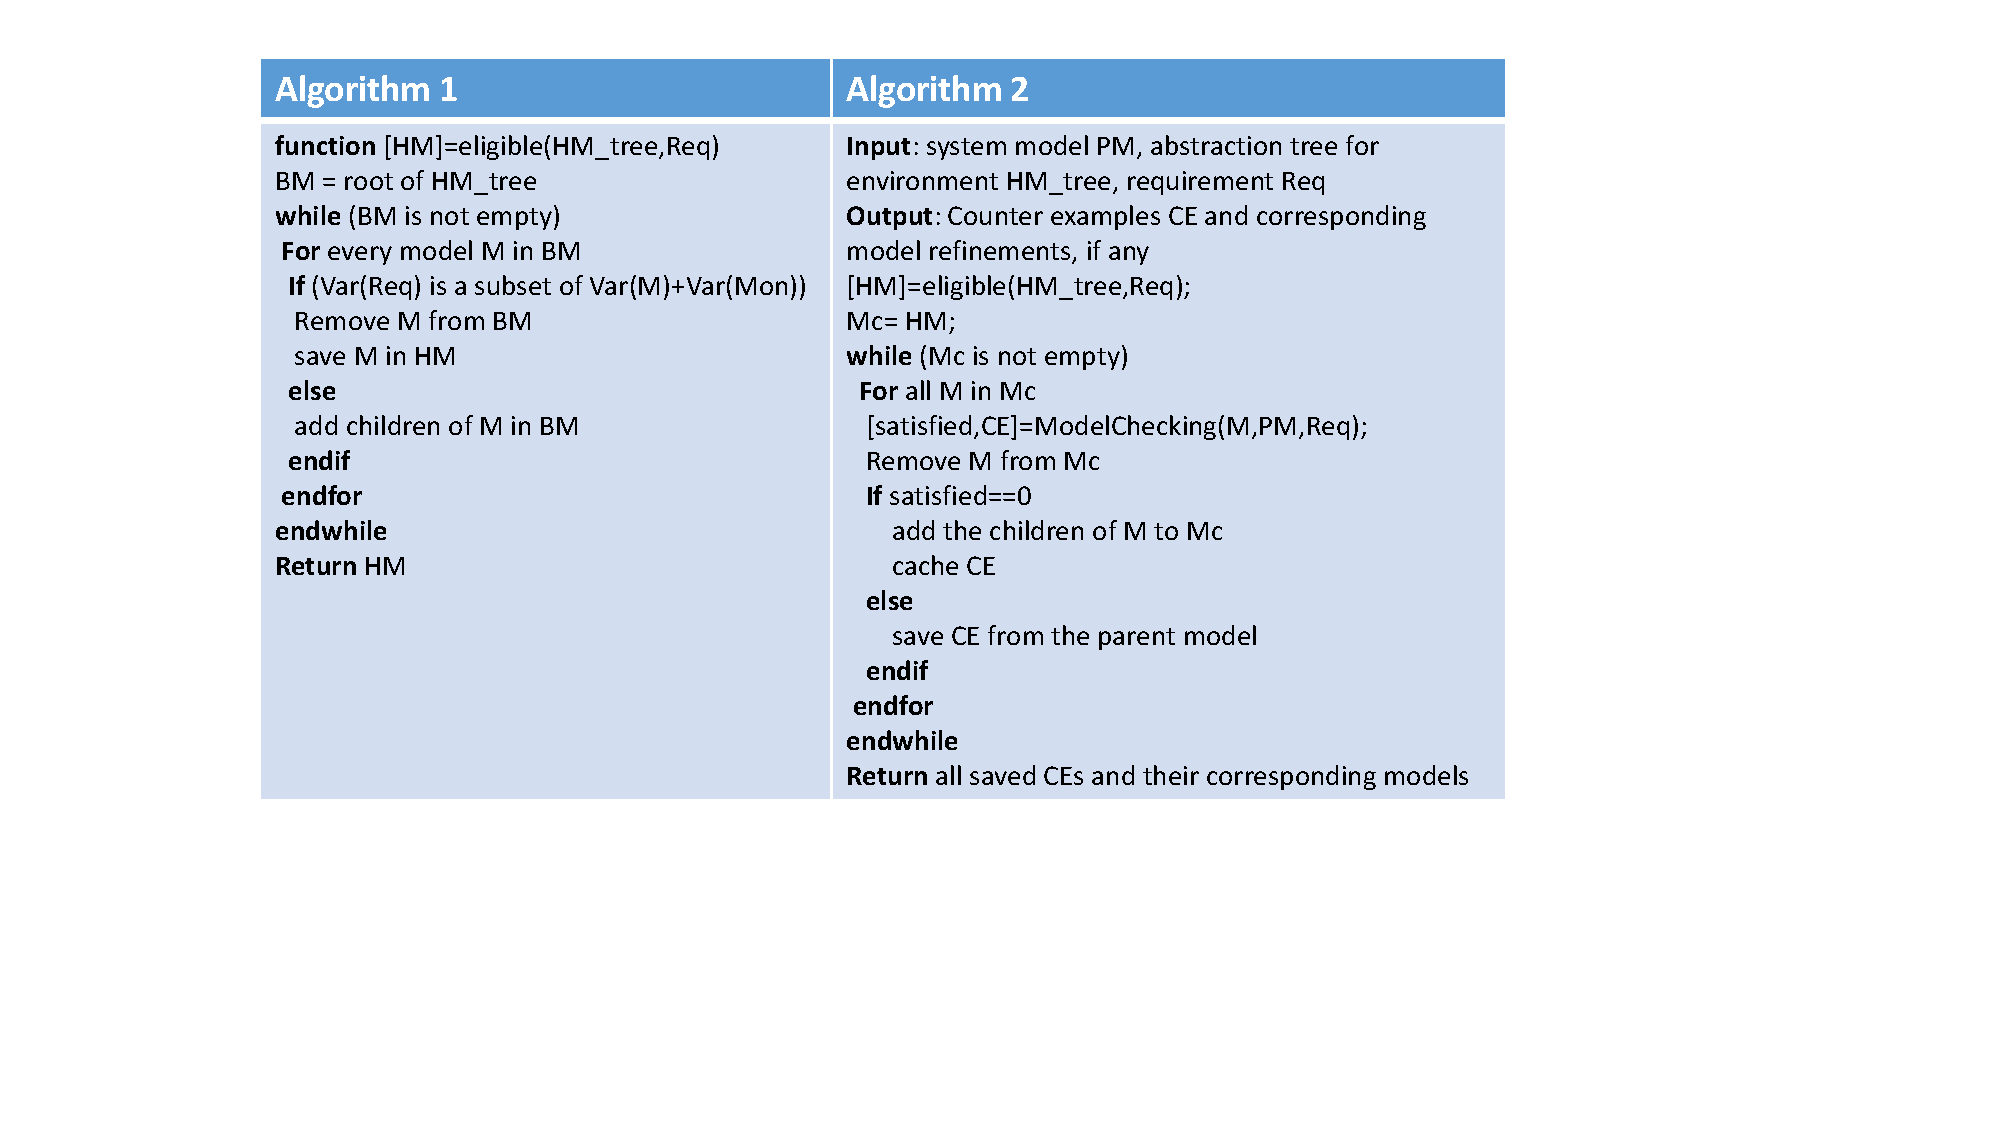
\includegraphics[width=0.9\textwidth]{figs/algorithm.pdf}
		%%\vspace{-5pt}
		%\caption{\small Algorithms for closed-loop model checking with abstraction tree}
		  %\vspace{-10pt}
		%\label{fig:algorithm}
%\end{figure}
Model checking is run on these models. 
When a run returns a violation, it returns an abstract counter-example $\delta_{cex}$, along with the heart model $M_{cex}$ that generated it.
For each such violation, we search the tree for the most concrete descendant of $M_{cex}$ that still displays a counter-example to $Req$.
This is then provided to the physician along with the counter-example.
The detailed implementation of the algorithm can be found in \cite{regar_tech}.
%Algorithm 2 (\figref{algorithm}) describes the process for closed-loop model checking with an abstraction tree.


%The most abstract model in the abstraction tree is built to cover the input space to the device as much as possible, thus it may not have enough details to constrain the behaviors of the model according to the constraints in the requirement. Thus the first step of closed-loop model checking is to select the most abstract models which are appropriate for the requirement. A model $M$ is appropriate for a requirement $Req$ if the environment transitions mentioned in the requirement, denoted as $EnvT(Req)$, is a subset of the environment transitions associated with the model $EnvT(M$). The following algorithm finds the most abstract heart models in the abstraction tree $HM\_tree$ that are appropriate for a requirement $Req$.
%\begin{Verbatim}
%Algorithm 1
%function [HM]=eligible(HM_tree,Req)
%BM = root of HM_tree
%while (BM is not empty)
 %For every model M in BM
  %If (Var(Req) is a subset of Var(M)+Var(Mon))
   %Remove M from BM
   %save M in HM
  %else
   %add children of M in BM
  %endif
 %endfor
%endwhile
%Return HM
%\end{Verbatim}
%BM = all models in HM_tree with all Prop(Req)
%For all M in BM
 %while (in the parent of M no behavior in Prop(Req) is abstracted with other behaviors)
	 %M = parent of M
 %endwhile
 %save M in HM
 %endfor

%\begin{Verbatim}
%Algorithm 2
%Input: system model PM, abstraction tree for environment HM_tree, requirement Req
%Output: Counter examples CE and corresponding model refinements, if any
%[HM]=eligible(HM_tree,Req);
%Mc= HM;
 %while (Mc is not empty)
  %For all M in Mc
   %[satisfied,CE]=ModelChecking(M,PM,Req);
	 %Remove M from Mc
	 %If satisfied==0
	  %add the children of M to Mc
		%cache CE
	%else
		%save CE from the parent model
	%endif
 %endfor
%endwhile
%Return all saved CEs and their corresponding models
%\end{Verbatim}
